% Packages utilisés~: fontenc, geometry, indentfirst, marvosym, esvect, wrapfig, physics, amssymb, mathtools, mhchem (v4), chemfig, adjustbox, enumitem, rsfso, cancel, makecell, subcaption, multicol, tikz, fancyhdr, lastpage, siunitx, tcolorbox, ifthen, caption, multirow, float.


\documentclass{article}
\usepackage[T1]{fontenc}
\usepackage[a4paper, margin=2cm]{geometry}
\usepackage{indentfirst} %indente qu'après un titre
\usepackage{marvosym} %symbol de la main qui écrit
\usepackage{esvect} %jolis vecteurs
\usepackage{wrapfig} %figures wrapped
\usepackage{physics} % macros de Physique
\usepackage{amssymb} % Symboles de Maths
\usepackage{mathtools} % Maths
\usepackage[version=4]{mhchem} % écrire des formules de chimie plus facilement
\usepackage{chemfig} % traçage de molécules
\usepackage{adjustbox} % pour les tableaux trop larges
\usepackage{enumitem} % pour garder un itemize et la ligne qui précède
\usepackage[scaled=1.1,scr]{rsfso} %pour les fontes scr 
\usepackage[makeroom]{cancel} %barrer des choses en diagonale (e.g. C2 §VIII.7)
\usepackage{makecell} %cases de tableau de plusieurs lignes
\usepackage{subcaption} %mettre deux figures à côté
\usepackage{multicol}

% TikZ
\usepackage{tikz} % Outil de dessin TikZ
\usetikzlibrary{positioning, decorations, decorations.pathmorphing, svg.path, calc}
\usepackage{pgfplots}
\pgfplotsset{compat=1.17}


\newcommand{\serpeg}{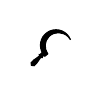
\begin{tikzpicture}[scale=0.05, rotate=90] %Dessin serpe gauloise
    \draw[fill=black] svg "m 85.80084559909016,214.0848263194619 -2.06515398583127,10.6699622601283 C 63.40206828227082,245.1959395037747 34.8434652071972,311.9906290729065 11.3692540264214,288.5164178921307 -12.10495715435405,265.0422067113552 54.64670837340594,236.4405795949098 75.08785929759045,216.1069562639218 l 10.71298630149971,-2.0221299444599 z";
    \draw[fill=black] svg "m 108.7419167440706,206.736972338917 -19.8340830722545,19.8340830722545 c 1.52410126960524,2.0394970349658 1.73127876250413,4.4641831949897 0.38721637234333,5.8082455851505 -1.5360713030409,1.536071303041 -4.54941029245121,1.0437150858417 -6.71175045395158,-1.1186250756586 L 68.55746210310377,217.2348384335593 c -2.16234016150031,-2.1623401615003 -2.61167233732806,-5.1326551095392 -1.07560103428716,-6.6687264125801 1.34406239016084,-1.3440623901608 3.76874855018474,-1.1368848972619 5.80824558515053,0.3872163723434 l 19.83408307225447,-19.8340830722546 15.61772701784898,15.617727017849 z";
    \draw[fill=black] svg "m 235.6535816959719,31.9640591939666 c 43.897708386389,43.897708386389 43.8977083863892,115.0331004398762 0,158.930808826265 -43.7245047247137,43.724504724714 -114.4767693137891,43.8957526893702 -158.41452032980723,0.5162884964578 l 16.95147230036508,-20.5654917755697 c 38.81906059246856,27.569114427687 92.07923865044546,24.7740577145076 125.80229697022164,-8.9490006052689 C 257.7671841813877,124.1223105912145 256.7199821471888,61.89341216770936 217.6695324026912,22.84296242321181 211.1465363002555,16.3199663207761 203.9694091953853,10.84862686886356 196.3726319238062,6.450802660676091 210.6929035158315,11.9233868411129 224.1124996231,20.42297712109476 235.6535816959719,31.9640591939666 z";
\end{tikzpicture}}

\newcommand{\nez}{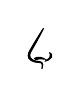
\begin{tikzpicture}[scale=0.0015] %Dessin sens Physique
    \draw[fill=black] svg "M5613.5,4620.6C4873.8,3491.5,3821,1773.4,2823,69c-547.9-935.4-655.5-1207.4-655.5-1673.1c0-238.7,35.2-403.1,117.4-571.4c240.7-483.3,771-821.9,1540-982.3c324.8-66.5,526.4-90,964.7-107.6c332.7-11.7,391.4-19.6,461.8-56.7c107.6-54.8,189.8-152.6,244.6-291.6c43-103.7,47-140.9,45-455.9c0-272-9.8-381.6-41.1-528.3c-23.5-101.8-39.1-189.8-35.2-191.8c3.9-3.9,33.3,74.4,64.6,176.1c209.4,653.6,176.1,1129.1-97.8,1375.7c-135,121.3-264.2,164.4-569.4,187.9c-630.1,47-1164.3,172.2-1569.4,367.9c-628.1,305.3-886.4,753.4-763.2,1326.7c64.6,311.1,129.2,444.2,649.7,1356.1C4143.9,1691.2,4893.3,3061,5525.4,4295.8c303.3,591,364,714.2,352.2,714.2C5873.7,5010,5754.4,4833.9,5613.5,4620.6z";
    \draw[fill=black] svg "M7407.9-968.2c-3.9-5.9,7.8-72.4,29.4-150.7c86.1-332.7,60.7-731.8-62.6-947.1c-68.5-115.5-236.8-293.5-405-422.7c-125.2-95.9-428.6-285.7-546-342.4c-70.4-33.3-90-64.6-39.1-64.6c58.7,0,495.1,154.6,636,225c342.5,172.2,596.8,401.2,739.7,665.3c70.5,133.1,72.4,142.9,72.4,342.5s-1.9,213.3-74.4,356.2C7664.2-1114.9,7458.8-917.3,7407.9-968.2z";
    \draw[fill=black] svg "M4261.3-2026.8c-164.4-35.2-471.6-185.9-536.2-264.2c-109.6-129.2-43.1-197.7,232.9-242.7c219.2-35.2,250.5-31.3,471.6,58.7c86.1,37.2,230.9,76.3,320.9,90c211.3,29.3,645.8,13.7,1074.3-41.1c174.2-23.5,322.9-37.2,328.8-31.3c62.6,62.6-634,340.5-1056.7,420.7C4848.3-1987.7,4460.9-1983.8,4261.3-2026.8z";
\end{tikzpicture}}


% Pied de page et en-tête
\usepackage{fancyhdr}
\usepackage{lastpage}

% Style de première page (sans header)
\fancypagestyle{plainsh}{
    \fancyhf{}%
    \renewcommand{\headrulewidth}{0.0pt}
    \cfoot{\footnotesize Page \textbf{\thepage}\ sur \textbf{\pageref{LastPage}}}
}

% style général
\makeatletter
\fancypagestyle{plain}{
    \fancyhf{}%
    \setlength{\headheight}{14.0pt} 
    \fancyhead[R]{\large{\acronyme{} -- \@title}}
    \fancyhead[L]{\large{MP1, 2021-2022}}
    \cfoot{\footnotesize Page \textbf{\thepage}\ sur \textbf{\pageref{LastPage}}}
}
\makeatother

% choix du style général
\pagestyle{plain}


%titres
\renewcommand{\abstractname}{Introduction}
\usepackage{sectsty}
\renewcommand{\thesection}{\Roman{section}.}
\renewcommand{\thesubsection}{\thesection\ \arabic{subsection})}
\renewcommand{\thesubsubsection}{\thesection\ \arabic{subsection})\ \alph{subsubsection})}

%Définition de la taille \HUGE
\usepackage{fix-cm}
\makeatletter
\newcommand\HUGE{\@setfontsize\Huge{50}{60}} 
\makeatother

% Personnalisation du titre
\makeatletter
\renewcommand\maketitle{
    \allsectionsfont{\sffamily}
    \thispagestyle{plainsh}
    \vspace*{2cm}
    \begin{center}
        \begin{minipage}{0.1\linewidth}   
            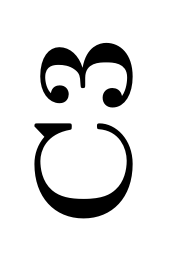
\begin{tikzpicture}
                \node [rotate=90] {\HUGE\textbf{\acronyme}}; % Référence du chapitre
            \end{tikzpicture}
        \end{minipage}
        \hspace{0.5em}
        \begin{minipage}{0.8\linewidth}
            {\raggedright
            {\Huge \bfseries \sffamily \@title }\\[0.25ex]
            {\LARGE \bfseries \itshape \soustitre}\\[1ex]
            {\Large  \@author}\\[4ex]}  
        \end{minipage}
    \end{center}
    \vspace{0.5cm}
}
\makeatother

% package pour les unités SI
\usepackage[load-configurations = abbreviations]{siunitx}
\sisetup{locale=FR, inter-unit-product=\ensuremath{{\cdot}}, detect-all, retain-explicit-plus}
\DeclareSIUnit{\ions}{\mathrm{ions}}

% cases

\usepackage{tcolorbox} %Pour les boxes de coleur
\tcbuselibrary{skins, breakable}
\usepackage{ifthen} % algorithmique

\definecolor{lav}{HTML}{800080}
\newtcolorbox{enonce}[1][]{%
    enhanced, attach boxed title to top left=
{xshift=-2mm,yshift=-2mm}, boxed title style={size=small,colback=blue!80}, breakable,colframe=blue!80,colback=blue!10, title={#1}
}

\newtcolorbox{remarque}[1][]{%
    enhanced, attach boxed title to top left=
{xshift=-2mm,yshift=-2mm}, boxed title style={size=small,colback=lav}, breakable,colframe=lav,colback=lav!10, title={#1}
}

\newtcolorbox{important}[1][]{%
    enhanced, attach boxed title to top left=
{xshift=-2mm,yshift=-2mm}, boxed title style={size=small,colback=red!75}, breakable,colframe=red!75,colback=red!10, title={#1}
}

% Types d'écrits
\newtcolorbox{tableau}[1][]{% %ce qu'il faut recopier au tableau
    grow to left by=0.5cm, enhanced, frame hidden, left=1.25cm, right=0cm, borderline west = {0.5pt}{1cm}{red, dashed}, colback=white, breakable, segmentation style={}, overlay={%
        \ifthenelse{\value{tcbbreakpart}=1}{% seulement pour le premier morceau
            \begin{tcbclipframe}
                \coordinate (X) at ([xshift=5mm,yshift=-5mm]frame.north west);
                \node[inner sep=1mm, color=black, font=\bfseries] at (X) {\LARGE{\WritingHand}};
            \end{tcbclipframe}
        }{}
    }
}

\newtcolorbox{appnum}[1][]{% %application numérique
    grow to left by=0.5cm, enhanced, frame hidden, left=1.25cm, right=0cm, borderline west = {0.4pt}{1cm}{red, decoration = {zigzag, segment length = 2mm, amplitude = 0.4mm}}, opacityfill=0, breakable, segmentation style={} , overlay={%
        \ifthenelse{\value{tcbbreakpart}=1}{% seulement pour le premier morceau
            \begin{tcbclipframe}
                \coordinate (X) at ([xshift=5mm,yshift=-5mm]frame.north west);
                \node[inner sep=1mm, color=black, font=\bfseries] at (X) {\serpeg};
            \end{tcbclipframe}
        }{}
    }
}

\newtcolorbox{sensphy}[1][]{% %Discussion physique~!
    grow to left by=0.5cm, enhanced, frame hidden, left=1.25cm, right=0cm, borderline west = {0.8pt}{1cm}{red, dotted}, opacityfill=0, breakable, segmentation style={} , overlay={%
        \ifthenelse{\value{tcbbreakpart}=1}{% seulement pour le premier morceau
            \begin{tcbclipframe}
                \coordinate (X) at ([xshift=5mm,yshift=-5mm]frame.north west);
                \node[inner sep=1mm, color=black, font=\bfseries] at (X) {\nez};
            \end{tcbclipframe}
        }{}
    }
}

\newtcolorbox{attention}[1][]{%
    grow to left by=0.5cm, enhanced, frame hidden, left=1.25cm, right=0cm, borderline west = {0.5pt}{1cm}{red}, opacityfill=0, breakable, segmentation style={} , overlay={%
        \ifthenelse{\value{tcbbreakpart}=1}{% seulement pour le premier morceau
            \begin{tcbclipframe}
                \coordinate (X) at ([xshift=5mm,yshift=-5mm]frame.north west);
                \node[inner sep=1mm, color=black, font=\bfseries] at (X) {\large{\fontencoding{U}\fontfamily{futs}\selectfont\char 66\relax}};
            \end{tcbclipframe}
        }{}
    }
}

\newenvironment{Figure}
  {\par\medskip\noindent\minipage{\linewidth}}
  {\endminipage\par\medskip}


% esthétique
\let\oldref\ref
\renewcommand{\ref}[1]{(\oldref{#1})}
\newcommand{\ds}{\displaystyle}
\usepackage{caption}
\usepackage{multirow}
\newcommand{\Dr}{\Delta_{\mathrm{r}}}
\newcommand{\Df}{\Delta_{\mathrm{f}}}
\renewcommand{\arraystretch}{1.5} % change la hauteur des cases des tableaux
\usepackage{float}


% commandes corps de texte
\newcommand{\ext}{\text{ext}}
\newcommand{\cste}{\text{cste}}
\newcommand{\EI}{\mathrm{EI}}
\newcommand{\EF}{\mathrm{EF}}
\newcommand{\rev}{\text{rév}}
\newcommand{\fp}{{\substack{\text{forces}\\\mathclap{\text{pressantes}}}}}
\newcommand{\pg}{\substack{\text{phase}\\\text{gazeuse}}}
\newcommand{\tprod}{\text{prod}}
\newcommand{\creee}{\text{créée}}
\renewcommand{\th}{\mathrm{th}}
\newcommand{\echangee}{\text{échangée}}
\newcommand{\Tz}{T_0 = \SI{298}{K}}
\newcommand{\Pz}{P^\circ = \SI{1,00}{bar}}
\newcommand{\cz}{c^\circ = \SI{1,00}{\mole\per\liter}}
\newcommand{\albe}{{\alpha \rightarrow \beta}}
\newcommand{\equi}{\text{eq.}}
\newcommand{\gaz}{\text{gaz}}

\newcommand{\acronyme}{C3}
\title{Sens d'évolution d'un système chimique}
\newcommand{\soustitre}{Déplacement, rupture d'équilibre et transformation totale}
\author{Guillaume \textsc{Saget},\\Professeur de Sciences Physiques au Lycée Champollion}

% Pour gérer la version support de cours et version entière
\newboolean{support}
\setboolean{support}{false} %changer sur true pour remplacer toutes les parties du tableau par "à faire"

\ifthenelse{\boolean{support}}
{\renewenvironment{tableau}
    {\begin{center}
        \textbf{À faire}
    \end{center}\comment}
    {\endcomment}}
{}

\begin{document}
\maketitle

\begin{abstract}
    Ce chapitre est consacré à l’évolution spontanée d’un système chimique~; moult questions se posent alors~: l’état d’équilibre chimique est-il toujours atteint lorsque l’évolution cesse~? Qu’appelle-t-on une transformation totale~? Comment reconnaître si une variable intensive est ou non un paramètre d’influence (appelé facteur d’équilibre) d’un équilibre chimique~? Quelles sont les lois de modération~? 
	Afin de répondre à ces questions, nous serons amenés à recenser les variables intensives pertinentes de description du système à l'équilibre pour en déduire la variance ou le nombre de degrés de liberté de celui-ci.
\end{abstract}

\section{Affinité chimique, enthalpie libre de réaction  et sens d’évolution (spontanée) d’un système chimique}
\subsection{Hypothèses de travail}
Soit un système de $N$ constituants siège d'une transformation chimique modélisée par l'équation de réaction $\sum_i \nu_i B_i = 0$ ($\nu_i$ le nombre stœchiométrique algébrique). La transformation chimique est monobare, monotherme, isobare, isotherme.

\subsection{Rappels}
\subsubsection{Enthalpie libre de réaction $\Dr G$}
\begin{tableau}
    Pour $G(T,P,n_1,\dots,n_N)$~:
    \begin{equation*}
        \dd{G} = \underbrace{\pdv{G}{T}}_{-S}\dd{T} + \underbrace{\pdv{G}{P}}_{V}\dd{P} + \sum_{i=1}^N \underbrace{\pdv{G}{n_i}}_{\mu_i}\bigg)_{T,P,n_i\neq n_j}\dd{n_i}
    \end{equation*}
    Via un zepto-tableau d'avancement, $n_i(t) = n_i(t=0) + \nu_i \xi$.\\
    Durant $\dd{t}$, $n_i(t)$ a varié de façon élémentaire de $\dd{n_i} = \nu_i\dd{\xi}$. Donc~:
    $$\dd{G} = -S\dd{T} + V\dd{P} + \sum_{i=1}^N \nu_i\pdv{G}{n_i}\bigg)_{T,P,n_i\neq n_j}\dd{\xi}$$
    On en déduit donc~:
    \begin{enonce}[Quatrième identité fondamentale de la thermochimie]
    \begin{equation}\label{id4}
        \dd{G} = V\dd{P} - S\dd{T} + \sum_i \nu_i\mu_i\dd{\xi}
    \end{equation}
    \end{enonce}
    \tcbline
    Avec $G(T,P,\xi)$~:
    \begin{equation*}
        \dd{G} = \pdv{G}{T}\dd{T} + \pdv{G}{P}\dd{P} + \underbrace{\pdv{G}{\xi}}_{\Dr G}\dd{\xi}
    \end{equation*}
    Pour une transformation isobare ($\dd{P}= 0$) et isotherme ($\dd{T} =0$),
    \begin{enonce}
        \begin{equation}\label{troputile}
            \dd{G} = \Dr G\times \dd{\xi}
        \end{equation}
    \end{enonce}
\end{tableau}
\subsection{Enthalpie libre standard de réaction $\Dr G^\circ$}
\begin{enonce}
    C’est la valeur de l’enthalpie libre de réaction lorsque tous les constituants sont dans leur état standard. Elle ne dépend que de la température $T$~:
    $$\Dr G^\circ(T) = \sum_i \nu_i\mu_i^\circ(T)$$
\end{enonce}
\begin{tableau}
    \textbf{Démonstration}\\
    Pour une transformation isobare ($\dd{P}= 0$) et isotherme ($\dd{T} =0$), on a~:
    $$\dd{G} \overset{\ref{id4}}{=} \sum_i\nu_i \dd{\xi} \overset{\ref{troputile}}{=} \Dr G\dd{\xi}$$
    \begin{important}
    \begin{equation}\label{drgiso}
        \xRightarrow[]{\dd{\xi}\neq 0} \Dr G = \sum_i \nu_i\mu_i
    \end{equation}
    \end{important}
    Lorsque tous les constituants sont dans leur état standard, on a~:
    \begin{important}
    \begin{equation*}
        \Dr G^\circ(T) = \sum_i \nu_i\mu_i^\circ(T)
    \end{equation*}
    \end{important}
\end{tableau}
\subsection{Enthalpie libre, affinité chimique et sens d’évolution}
\subsubsection{Critère de l’évolution spontanée}
\begin{tableau}
    \begin{enonce}[Rappel]
        Le critère de l'évolution spontanée prédit que $\mathscr{A}\dd{\xi} >0$.
    \end{enonce}
    \textbf{Conséquences.}
    \begin{itemize}
        \item Si $\mathscr{A}>0 \iff \Dr G<0$. Puisque $\mathscr{A}\dd{\xi} >0$, $\dd{\xi} >0 \implies \xi \nearrow$ donc le système chimique évolue dans le sens direct.
        \item Si $\mathscr{A}<0 \iff \Dr G>0$. Puisque $\mathscr{A}\dd{\xi} >0$, $\dd{\xi} <0 \implies \xi \searrow$ donc le système chimique évolue dans le sens indirect.
    \end{itemize}
\end{tableau}
\subsubsection{Condition d’équilibre chimique}
\begin{important}
    Le système est à l'équilibre chimique si et seulement si $\Dr G=0$.
\end{important}


\section{Utilisation de l’enthalpie libre de réaction et de l’affinité chimique}
\subsection{Calcul de l’enthalpie libre de réaction et de l’affinité à partir des potentiels chimiques ou des activités}
$$\Dr G = \sum_i \nu_i \mu_i$$

\subsection{Définition du quotient de réaction $Q_r$}
\begin{tableau}
    D'après le cours C2, on a vu qu'on peut toujours\footnotemark{} marquer~:
    $$\mu_i = \mu_i^\circ + RT\ln(a_i)$$
    Il vient~:
    \begin{align*}
        \Dr G &= \mu_i \nu_i\mu_i^\circ + RT\sum\nu_i \ln(a_i)\\
        &=\Dr G^\circ(T) + RT\ln\left[\prod_{i=1}^N a_i^{\nu_i}\right]
    \end{align*}
    \begin{important}
        On pose donc $Q_r=\ds\prod_{i=1}^N a_i^{\nu_i}$ le \textit{quotient de réaction} du système siège d'une transformation chimique.
    \end{important}
    Par définition de la constante d'équilibre $K^\circ(T)$~:
    $$\Dr G^\circ(T) + RT\ln\big(K^\circ(T)\big)=0 \implies \Dr G = -RT\ln K^\circ + RT\ln Q_r$$
    Et finalement,
    \begin{important}
        \begin{equation}\label{drgqrk}
            \Dr G = RT\ln\left(\frac{Q_r}{K^\circ}\right)
        \end{equation}
    \end{important}
\end{tableau}
\footnotetext{En vrai, NON~!}

\subsection{Equilibre chimique~: loi d’action des masses (relation de Guldberg et Waage)}
D'après \ref{drgqrk}, à l'équilibre chimique,
$$\Dr G = 0 \iff K^\circ(T) = Q_{r,\equi}$$
\begin{enonce}[Loi d'action des masses]
    $$Q_{r,\equi} = \prod_{i=1}^N a_i^{\nu_i} = K^\circ(T)$$
\end{enonce}
\subsection{Déduction du sens de l’évolution spontanée  par détermination du signe de l’enthalpie libre de réaction à partir de la comparaison de $K^\circ$ et $Q_r$}
\begin{tableau}
    D'après \ref{drgqrk},
    \begin{itemize}
        \item Si la réaction évolue spontanément dans le sens direct, $\mathscr{A}>0 \iff \Dr G<0 \iff Q_r < K^\circ$.
        \begin{figure}[H]
            \centering
            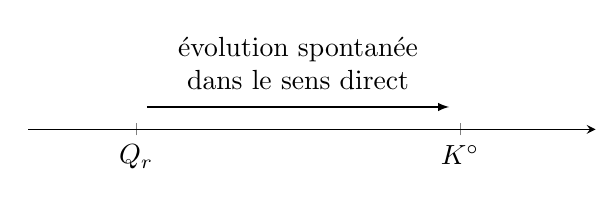
\begin{tikzpicture}
            \begin{axis}[clip = false, axis lines = left, axis line style={shorten >=-10pt}, axis y line=none, xmax=5, ymax=3, xmin=0, ymin=0, xtick={1,4}, xticklabels={$Q_r$,$K^\circ$}, ytick=\empty,  >=latex]
            \draw [->] (1.1,0.15) --node [above, align=center, yshift=1mm]{évolution spontanée\\dans le sens direct} (3.9,0.15);
        \end{axis}
        \end{tikzpicture}
        \end{figure}
        \item Si la réaction évolue spontanément dans le sens indirect, $\mathscr{A}<0 \iff \Dr G>0 \iff Q_r > K^\circ$.
        \begin{figure}[H]
            \centering
            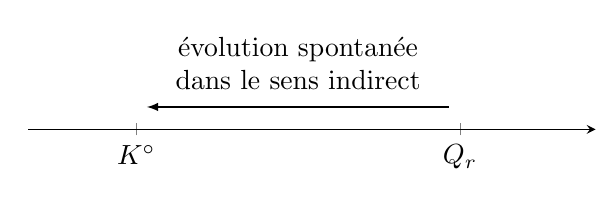
\begin{tikzpicture}
            \begin{axis}[clip = false, axis lines = left, axis line style={shorten >=-10pt}, axis y line=none, xmax=5, ymax=3, xmin=0, ymin=0, xtick={1,4}, xticklabels={$K^\circ$,$Q_r$}, ytick=\empty,  >=latex]
            \draw [<-] (1.1,0.15) --node [above, align=center, yshift=1mm]{évolution spontanée\\dans le sens indirect} (3.9,0.15);
        \end{axis}
        \end{tikzpicture}
        \end{figure}
    \end{itemize}
\end{tableau}
\section{Système en fin d’évolution}
\subsection{Rappels de C2~: variance ou nombre de degrés de liberté d’un système physico-chimique}
\subsubsection{Définition}
\begin{enonce}
    La \textit{variance} ou nombre de degrés de liberté d’un système physico-chimique est le nombre de paramètres intensifs indépendants que l’expérimentateur peut faire varier simultanément sans entraîner la rupture de l’équilibre chimique (Cf paragraphe suivant pour la définition de la rupture d’équilibre).
\end{enonce}

\textbf{Nota Bene.} Il existe deux types de paramètres intensifs descriptifs du système~:
\begin{itemize}
    \item les paramètres intensifs « physiques » $T$ (température du système) et $P$ (pression totale du système)~;
    \item les paramètres intensifs de composition de phase décrits par les fractions molaires $x_i=\frac{n_i}{n}$ ou des pressions partielles $p_i$ s'il s'agit de constituants gazeux.
\end{itemize}

\subsubsection{Règle des phases de Gibbs}
\begin{enonce}[Règle des phases de Gibbs (admise)]
    La variance $v$ se calcule comme suit~:
    $$v=2+n-\varphi-q-r$$
\end{enonce}
Avec~:
\begin{itemize}
    \item « $2$ » pour les variables intensives\footnote{\textbf{À nuancer dans le paragraphe \textsc{V.}}} $T$ et $P$~;
    \item $n$ (ou noté $c$) est le nombre de constituants physico-chimiques~;
    \item $\varphi$ le nombre de phases~;
    \item $q$ le nombre de relations supplémentaires imposées par l'expérimentateur ou issues de la stœchiométrie~;
    \item $r$ le nombre d'équilibres chimiques indépendants.
\end{itemize}

\subsection{État d’un système en fin d’évolution (État final: EF)}
\subsubsection{Position du problème}
Lorsque l’évolution d’un système physico-chimique cesse, l’état final est atteint. Les équilibres mécanique et thermique sont atteints lors d’une transformation chimique monobare, monotherme ou isobare, isotherme. Qu’en est-il de l’équilibre chimique~? Réponse~: \textbf{L’état final n’est pas nécessairement un état d’équilibre chimique}.

\subsubsection{Critère d’atteinte de l’équilibre chimique à l’état final}
\begin{important}[Critère]
    L’état final (acronyme EF) correspond à un équilibre chimique (acronyme EQ) si et seulement si il y a coexistence dans le milieu réactionnel de tous les constituants intervenant dans l’équation de réaction.
\end{important}
\begin{tableau}
    \textbf{Conséquence}\\
    À l'état final (EF), on a $\dd{G}=0$. D'après \ref{troputile}, on a donc $\Dr G \times \dd{\xi}=0$.
    \begin{itemize}
        \item Si $\Dr G=0$, on atteint l'équilibre chimique, l'évolution cesse donc $\xi = \xi_\equi = \cste$. ($\EF=\EI$)
        \item Si $\dd{\xi} = 0$, alors $\xi = \xi_f$. L'évolution cesse mais $\Dr G(\xi=\xi_f) \neq 0$ donc l'équilibre chimique n'est pas atteint. On parle de \textbf{rupture d'équilibre}.
    \end{itemize}
\end{tableau}
\subsubsection{Définition~: réaction totale ou complète}
\begin{enonce}
    Une \textit{réaction} est dite \textit{totale} ou complète ou quantitative si l’espèce limitante (réactif limitant si la réaction a lieu dans le sens direct ou produit limitant si la réaction a lieu dans le sens inverse) a disparu.
\end{enonce}

\subsubsection{Rupture d'équilibre}
On parle de rupture d’équilibre lorsque la réaction cesse sans qu’un état d’équilibre chimique soit instauré.\\
Fort des définitions précédentes, une \textbf{réaction totale} correspond nécessairement à une \textbf{rupture d’équilibre} et réciproquement.


\subsection{Des exemples de systèmes physico-chimique}
\subsubsection{Position du problème}

    Deux situations sont envisageables~: système homogène ou système hétérogène.
\begin{tableau}
    \begin{itemize}
    \item \textit{Système homogène}~: tous les constituants sont dans une même phase (par exemple en phase acqueuse).
    \item \textit{Système hétérogène}~: il existe plusieurs phases mises en jeu dans le mélange réactionnel.
\end{itemize}
\textbf{NB~:} Cinq solides (non-almagamés) représentent cinq phases différentes.
\end{tableau}

\subsubsection{Système homogène}
\begin{enonce}
    Un \textit{système homogène} est un système mettant une seule phase (mélange de gaz~: une seule phase gazeuse, des constituants en solution aqueuse (une phase aqueuse) ou encore un mélange de liquides miscibles~: une seule phase liquide).
\end{enonce}
En phase homogène (gazeuse, aqueuse ou liquide), toutes les espèces (réactifs et produits) sont présentes à l’état final. \textbf{Comme l’état d’équilibre chimique} correspond à l’\textbf{existence} dans le milieu réactionnel de tous les constituants intervenant dans l’équation de réaction (même si certains constituants sont en quantité infime), l’état final est un état d’équilibre chimique. \textbf{Il n’y a pas de rupture d’équilibre à envisager.}

\begin{remarque}[Remarque]
    Lorsque l’espèce limitante (réactif limitant ou produit limitant) est en quantité infinitésimale à l’état d’équilibre, on considère la réaction comme « totale » lors de l’écriture du tableau d’avancement mais elle ne \textbf{l’est rigoureusement pas} (car, répétons-le,  tous les constituants sont présents). On devrait parler de réaction « quasi-totale ». 
\end{remarque}

\subsubsection{Système hétérogène}
\begin{enonce}
    Un \textit{système hétérogène} est un système mettant en jeu une ou plusieurs phases condensées pures.
\end{enonce}
Certaines espèces (réactifs et produits)  peuvent disparaître à l’état final. Le calcul de la variance ou de la variance réduite (Cf. TD C3) du système physico-chimique peut s’avérer utile pour savoir si une rupture d’équilibre est envisageable. \textbf{Une rupture d’équilibre peut se produire pour les systèmes monovariants ($v = 1$) ou invariants ($v = 0$).}\\

\textbf{Exemple~:} Considérons la réaction ne mettant en jeu que des phases condensées pures (liquides non miscibles, solides) avec l’introduction de toutes les espèces (réactifs et produits).
\begin{tableau}
    \textbf{Exemple~: système hétérogène fermé de $N$ constituants qui forment chacun une phase condensée pure.}\\
    A priori, la règle des phases de Gibbs donne~:
    $$v=2+n-\varphi-r-q \overset{(\mathrm{AN})}{=} \underset{\mathclap{\substack{\downarrow\\ T,P}}}{2}+N-N-1-0=1$$
    En réalité, si la pression a une influence sur le mélange réactionnel, alors $\sum_i\nu_{i,\gaz} \neq 0$ et réciproquement. Dans ce cas, on dit que la pression est un facteur d'équilibre.\\
    Pour notre exemple, chaque constituant forme une phase condensée pure donc $\sum_i\nu_{i,\gaz} = 0$. Ainsi, $P$ n'est pas un paramètre d'équilibre.\\
    Ainsi, la règle des phases devient~:
    $$v=1+n-\varphi-r-q \overset{(\mathrm{AN})}{=} \underset{\mathclap{\substack{\downarrow\\ T,\cancel{P}}}}{1}+N-N-1-0=0$$
    Le système est invariant.\\
    \tcbline
    Travaillons à une température $T$. On a $K^\circ(T) = e^{\frac{-\Dr G^\circ}{RT}}$. Calculons le quotient de réaction. À l'EI, tous les constituants ont été introduits d'où pour tout $i\in \{1,\dots,N\}$, $a_i = 1$. Et finalement,
    $$Q_{r,\EI} = \prod_{i=1}^N a_i^{\nu_i} =1$$
    \textbf{Il y a trois cas à traiter~:}
    \begin{itemize}
        \item Si $Q_{r,\EI}=1 < K^\circ(T)$~: on sait d'après le critère de l'évolution spontanée que la réaction évolue spontanément dans le sens direct. Lors de la réaction, les réactifs s'épuisent. Tant que tous les constituants sont présents, leur activité vaut $1$ et le quotient de réaction vaut $Q_r = Q_{r,\EI} = 1$.\\
        Il existe une date $t_f$ à laquelle le réactif limitant disparaît mettant fin à la réaction chimique~: l'évolution cesse~; l'activité du réactif limitant vaut désormais $0$.
        $$Q_r(t) \xrightarrow[t\rightarrow t_f]{}+\infty\neq K^\circ(T)$$
        Donc $\EF \neq \EI$~: on a une rupture d'équilibre.
        \item Si $K^\circ(T) < Q_{r,\EI}=1$~: on sait d'après le critère de l'évolution spontanée que la réaction évolue spontanément dans le sens inverse jusqu'à épuisement du produit limitant.\\
        Il existe une date $t_f$ à laquelle le produit limitant disparaît du mélange réactionnel. À cette date, son activité est nulle.
        $$Q_{r}(t=t_f) = Q_{r,\EF} = 0 \neq K^\circ(T)$$
        Donc $\EF = \EI$.
        \item Si $K^\circ(T) = Q_{r,\EI}=1$~: on travaille à la température $T=T_0$ pour laquelle $\Dr G^\circ(T_0) = 0 \iff K^\circ(T_0)=1$. ($T_0$ est appelée \textit{température d'inversion})\\
        Ici, $Q_{r,\EI} = 1 = K^\circ(T_0)=1$. Le système est à l'équilibre chimique ($\mathscr{A}=0$). Il n'y a pas d'évolution macroscopique.
    \end{itemize}
\end{tableau}
\textbf{En conclusion (pour cet exemple):}
\begin{itemize}
    \item Si $Q_r = 1 < K^\circ(T)$~: à la température $T$, le système évolue dans le sens direct jusqu’à  l’épuisement du réactif limitant. L’état final n’est pas un état d’équilibre chimique. \textbf{La réaction est totale.}
    \item Si $K^\circ(T) < Q_r = 1$~: à la température $T$, le système évolue dans le sens inverse jusqu’à  l’épuisement du « réactif limitant » (c’est l’un des produits de la réaction). L’état final n’est pas un état d’équilibre chimique. \textbf{La réaction est totale.}
    \item Si $K^\circ(T_0) = Q_r = 1$~: le système est à l’\textbf{équilibre chimique} et c’est seulement à cette température $T_0$ qu’il y a coexistence des phases condensées. La réaction n’est donc pas totale. A cette température $T_0$, appelée température d’inversion, $\Dr G^\circ(T_0) = 0$.
\end{itemize}
%On a ici répétition entre ce qu'on avait marqué et le support de cours et je ne vois pas comment trier.

\begin{remarque}[Remarque]
    Notons qu’une réaction peut être totale même avec $K^\circ(T_0)\approx 1$  (Cf. exemple précédent)~!!!
\end{remarque}

\textbf{En résumé~:}\\
Le problème est de savoir si \textbf{tous les constituants sont présents ou non} à la fin de l’évolution du système.
\begin{itemize}
    \item Si c’est le cas, l’EF est un état d’équilibre chimique à la température $T_0$~: $Q_{r,\equi} = K^\circ(T_0)$.
    \item Si une phase condensée a disparu, l’équilibre chimique ne peut être atteint ($Q_r = 0$ voire non défini\footnote{On peut calculer $Q_{r,\EF}$ lorsqu’il reste encore un « grain » d’espèce limitante de façon à ce que le calcul de l’affinité chimique ou de l’enthalpie libre de réaction à l’EF soit possible (Cf. exercice n°10 du TD C3).})~: il y a rupture d’équilibre et l’état final n’est pas un état d’équilibre chimique. À cette température $T_0$, la réaction est alors \textbf{totale ou quantitative}.
\end{itemize}

\section{Rappels et cadre de travail}
\subsection{Déplacement ou rupture de l’équilibre chimique conduisant à une transformation totale}
L’état du système à l’équilibre chimique est parfaitement déterminé et on envisage une perturbation modérée de ce système.

La perturbation peut provenir de la modification d’un paramètre physique (pression ou température) ou d’un paramètre de composition du système (ajout d’un constituant inerte\footnote{Un constituant est dit inerte si ce n’est pas un des constituants participant à la transformation chimique. Dans le cas contraire, il est dit actif. Cette étude réalisée dans les anciens programmes n’est désormais plus au programme de MP... mais réintroduite dans notre cours millésimé 2019-2020 (du fait de la frénésie des banques de concours à faire tout azimut des entorses au programme... Rappelez-vous~: il n’y a plus de programme en MP~!)} ou actif).

Pour réaliser cette étude, on considère le nouvel état du système après perturbation et on analyse, pour le système bloqué (avant toute réaction chimique donc) les valeurs relatives du quotient de réaction $Q_r'$ et de la constante d’équilibre $K^\circ(T)$ après la perturbation afin de prévoir le sens d’évolution.

À la suite de la perturbation, le système pourra évoluer vers un nouvel d’équilibre chimique. Tous les constituants du système demeurent présents dans le milieu après son évolution. C’est le cas des systèmes homogènes ou des systèmes hétérogènes dont le nombre de degrés de liberté (ou variance) est supérieure ou égal à deux. 

Mais l’évolution du système chimique peut aussi conduire, comme on le verra dans le TD C3 dans l’exercice de la dissociation du calcaire (le nombre de degrés de liberté vaut un pour ce système) à une rupture d’équilibre chimique (avec disparition d’un constituant formant une phase pure condensée) conduisant au \textbf{caractère total} de la transformation mise en jeu.

\subsection{Lois de modération}
\begin{important}
    Dans la plupart des cas, le système obéit à la \textit{loi de modération}~: son évolution tend à s’opposer à la perturbation qui l’a engendré, c’est-à-dire à en modérer les effets (lois de modération de Vant’Hoff, de Le Châtelier, ...).
\end{important}

\section{Modification d’un paramètre physique du système}
\subsection{Modification de la température du système}
\subsubsection{Position du problème}
Soit un système chimique initialement à l’équilibre chimique. On travaille à $\Tz$. On envisage une modification modérée de la température, à pression et composition constantes. À $T_0$,
$$K^\circ(T_0) = e^{\frac{-\Dr G^\circ(T_0)}{RT_0}}$$
\subsubsection{Loi de Van't Hoff}
\begin{enonce}[Loi de Van't Hoff]
    Une élévation modérée de température à pression constante et composition constantes entraîne une évolution du système dans le sens endothermique de la réaction.
\end{enonce}
\begin{tableau}
    \begin{attention}
        Il faut que la température $T=T_0$ soit un paramètre d'équilibre, i.e. $\Dr H^\circ(T=T_0) \neq 0$. En effet, si $\Dr H^\circ(T=T_0) = 0$, la réaction est athermique et $T$ n'est pas un paramètre d'équilibre.
    \end{attention}
    \textbf{Démonstration} à partir de~: $\ds\dv{(\ln K^\circ)}{T} = \frac{\Dr H^\circ}{RT^2}$.\\
    
    Augmentons la température du système~: $T \nearrow \implies \dd{T}>0$.\\
    On passe de $T_0$ à $T_0+\dd{T}$. D'après la relation de Van't Hoff~:
    \begin{align*}
        \dd(\ln K^\circ) &= \frac{\Dr H^\circ(T_0+\dd{T})}{R(T_0+\dd{T})^2}\dd{T}\\
        &\approx \frac{\Dr H^\circ}{RT_0^2}\underbrace{\dd{T}}_{>0}
    \end{align*}
    Il y a maintenant trois cas à étudier~:
    \begin{itemize}
        \item \textbf{Premier cas~: la réaction est endothermique (dans le sens direct)}\\
        On a ainsi $\Dr H^\circ(T_0) > 0$ et donc~:
        $$\dd(\ln K^\circ) = \frac{\Dr H^\circ}{RT_0^2}\dd{T} >0$$
        Donc $\ln K^\circ \nearrow$ lorsque $T \nearrow$ et ainsi $K^\circ \nearrow$ lorsque $T\nearrow$.\\
        Effet de la perturbation induite par l'augmentation de $T$~: nouvel état initial.
        \begin{itemize}
            \item Avant perturbation~: EQ. $Q_{r,\equi} = K^\circ(T_0)$.
            \item Perturbation appliquée~: $\EI'$. $Q_{r,\equi}'=Q_{r,\EI}'<K^\circ(T_0+\dd{T})$.
        \end{itemize}
        \begin{figure}[H]
            \centering
            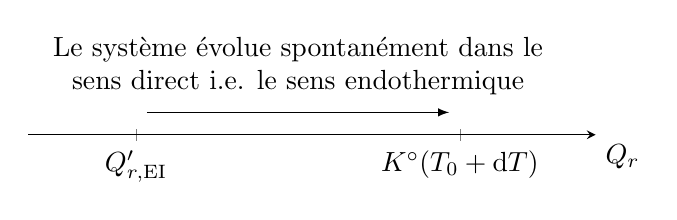
\begin{tikzpicture}
                \begin{axis}[clip = false, axis lines = left, axis line style={shorten >=-10pt}, axis y line=none, xmax=5, ymax=3, xmin=0, ymin=0, xtick={1,4}, xticklabels={$Q_{r,\EI}'$,$K^\circ(T_0+\dd{T})$}, ytick=\empty,  >=latex, xlabel=$Q_r$,every axis x label/.style={anchor=north east,at={(1.1,0)},xshift=10pt}]
                    \draw [->] (1.1,0.15) --node [above, align=center,yshift=1mm]{Le système évolue spontanément dans le\\sens direct i.e. le sens endothermique} (3.9,0.15);
                \end{axis}
            \end{tikzpicture}
        \end{figure}
        \item \textbf{Second cas~: la réaction est exothermique dans le sens direct (ou endothermique dans le sens inverse)}\\
        On a ainsi $\Dr H^\circ(T_0) < 0$ et donc~:
        $$\dd(\ln K^\circ) = \frac{\Dr H^\circ}{RT_0^2}\dd{T} <0$$
        Donc $\ln K^\circ \searrow$ lorsque $T \nearrow$ et ainsi $K^\circ \searrow$ lorsque $T\nearrow$.\\
        Effet de la perturbation induite par l'augmentation de $T$~: nouvel état initial.
        \begin{itemize}
            \item Avant perturbation~: EQ. $Q_{r,\equi} = K^\circ(T_0)$.
            \item Perturbation appliquée~: $\EI'$. $K^\circ(T_0+\dd{T})<Q_{r,\equi}'=Q_{r,\EI}'$.
        \end{itemize}
        \begin{figure}[H]
            \centering
            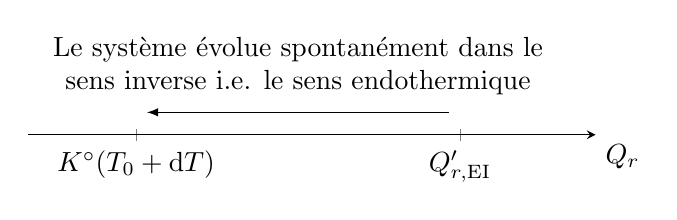
\begin{tikzpicture}
                \begin{axis}[clip = false, axis lines = left, axis line style={shorten >=-10pt}, axis y line=none, xmax=5, ymax=3, xmin=0, ymin=0, xtick={1,4}, xticklabels={$K^\circ(T_0+\dd{T})$,$Q_{r,\EI}'$}, ytick=\empty,  >=latex, xlabel=$Q_r$,every axis x label/.style={anchor=north east,at={(1.1,0)},xshift=10pt}]
                    %\draw [->] (1.1,-0.4) --node [below, align=center, yshift=-1mm]{Si le système évoluait spontanément dans le\\sens direct, il évoluerait dans le sens exothermique} (3.9,-0.4);
                    \draw [<-] (1.1,0.15) --node [above, align=center,yshift=1mm]{Le système évolue spontanément dans le\\sens inverse i.e. le sens endothermique} (3.9,0.15);
                \end{axis}
            \end{tikzpicture}
        \end{figure}
        \item \textbf{Troisième cas~: la réaction est athermique}\\
        On a ainsi $\Dr H^\circ(T_0) = 0$ et donc \textbf{la température n'est pas un facteur d'équilibre} lors d'une augmentation modérée de la température $T$. Finalement, la température n'a pas d'impact sur un éventuel déplacement de l'équilibre.
    \end{itemize}
    La loi de Van't Hoff est démontrée.
\end{tableau}
    \begin{important}[Conséquence]
        Pour une transformation endothermique (respectivement exothermique), l’équilibre chimique sera favorable aux produits à haute température (respectivement à basse température).
    \end{important}
\subsection{Modification de la pression du système}
    \subsubsection{Position du problème}
    Soit un système chimique initialement à l’équilibre chimique. On envisage une modification de la pression, à température et composition constantes.
    \subsubsection{Équilibre en phase condensée}
    Tant que l’on peut négliger l’influence de la pression sur le potentiel chimique en phase condensée, le quotient de réaction ne dépend pas de la pression~: la pression est sans influence sur l’équilibre chimique~; on dit que \textbf{la pression n’est pas un facteur d’équilibre}.
    \begin{important}
        Le nombre de degrés de liberté « physiques »  intervenant dans le calcul de la variance (ou nombre de degrés de liberté du système physico-chimique) via la règle des phases n’est plus égal à $2$ ($T$, $P$) mais à $1$ ($T$).
    \end{important}
    \begin{remarque}[Question]
        Pour une réaction chimique athermique, où tous les constituants sont en phase condensée, que vaut le nombre de degrés de liberté « physiques » du système~?
    \end{remarque}
        Puisque $T$ n'est pas un facteur d'équilibre et que $P$ non plus ($\sum_i \nu_{i,\gaz} =0$), la règle des phases devient~:
        $$v=\underset{\mathclap{\substack{\downarrow\\ \cancel{T,P}}}}{0}+n-\varphi-q-r$$
        
        \subsubsection{Système homogène ou hétérogène gazeux}
        \begin{enumerate}[label={\textsf{\textbf{\roman*)}}}]
            \item \textbf{\textsf{Position du problème}}\\
            Soit un système hétérogène contenant des constituants gazeux.
            \item \textbf{\textsf{Loi de le Châtelier}}
            \begin{enonce}[Loi de le Châtelier]
                Une élévation modérée de pression à température constante et composition constantes entraîne une évolution du système dans le sens d’une diminution du nombre total de moles gazeuses du milieu.
            \end{enonce}
            \begin{tableau}
                \textbf{Démonstration dans le cas où il existe une seule phase gazeuse}\\
                À l'équilibre chimique~:
                $$Q_{r,\equi} = \prod_ia_{i,\equi}^{\nu_{i,\gaz}} = K^\circ(T_0)$$
                On applique une perturbation~: en augmentant la pression, on a donc $\dd{P}>0$ et donc $Q_r$ est impacté.
                \begin{align*}
                    Q_i&=\prod_ia_i^{\nu_{i,\gaz}}=\prod_i \left(\frac{p_i}{P^\circ}\right)^{\nu_{i,\gaz}}=\prod_i \left(\frac{x_iP}{P^\circ}\right)^{\nu_{i,\gaz}}=\prod_i \left[\left(\frac{x_i}{P^\circ}\right)^{\nu_{i,\gaz}}\times P^{\nu_{i,\gaz}}\right]\\
                    &=\left[\prod_{i=1}^N \left(\frac{x_i}{P^\circ}\right)^{\nu_{i,\gaz}}\right]\times P^{\sum_i\nu_{i,\gaz}} = \cste \times P^{\Dr \nu_{\gaz}}\\
                    \implies \ln Q_r &= \ln(\cste) + \Dr \nu_{\gaz}\ln(P)\\
                    \implies \frac{\dd{Q_r}}{Q_r} &= \Dr \nu_{\gaz}\frac{\dd{P}}{P}
                \end{align*}
                En rappelant que $\dd{P} >0$ et $Q_r >0$, on étudie les trois cas suivants~:
                \begin{itemize}[label=\textbullet]
                    \item \textbf{Premier cas~: $\Dr \nu_{\gaz} >0$}\\
                    On a donc $\dd{Q_r} >0$ et donc $Q_r \nearrow$ lorsque $P \nearrow$. Nouvel état initial~: $Q_{r,\EI}'$.
                    \begin{figure}[H]
                        \centering
                        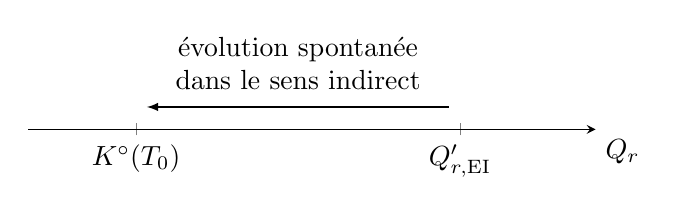
\begin{tikzpicture}
                            \begin{axis}[clip = false, axis lines = left, axis line style={shorten >=-10pt}, axis y line=none, xmax=5, ymax=3, xmin=0, ymin=0, xtick={1,4}, xticklabels={$K^\circ(T_0)$,$Q_{r,\EI}'$}, ytick=\empty,  >=latex, xlabel=$Q_r$,every axis x label/.style={anchor=north east,at={(1.1,0)},xshift=10pt}]
                                \draw [<-] (1.1,0.15) --node [above, align=center,yshift=1mm]{évolution spontanée\\dans le sens indirect} (3.9,0.15);
                            \end{axis}
                        \end{tikzpicture}
                    \end{figure}
                    D'après le critère de l'évolution spontanée, le système évolue spontanément dans le sens inverse, i.e. dans le sens où la phase gazeuse s'appauvrit.
                    \item \textbf{Second cas~: $\Dr \nu_{\gaz} <0$}\\
                    On a donc $\dd{Q_r} <0$ et donc $Q_r \searrow$ lorsque $P \nearrow$. Nouvel état initial~: $Q_{r,\EI}'$.
                    \begin{figure}[H]
                        \centering
                        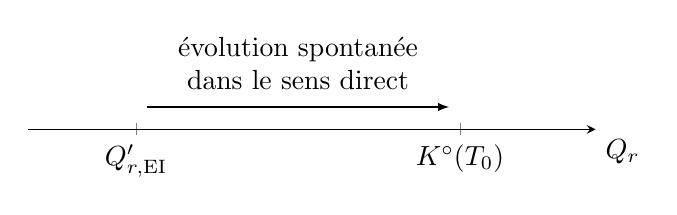
\begin{tikzpicture}
                            \begin{axis}[clip = false, axis lines = left, axis line style={shorten >=-10pt}, axis y line=none, xmax=5, ymax=3, xmin=0, ymin=0, xtick={1,4}, xticklabels={$Q_{r,\EI}'$,$K^\circ(T_0)$}, ytick=\empty,  >=latex, xlabel=$Q_r$,every axis x label/.style={anchor=north east,at={(1.1,0)},xshift=10pt}]
                                \draw [->] (1.1,0.15) --node [above, align=center,yshift=1mm]{évolution spontanée\\dans le sens direct} (3.9,0.15);
                            \end{axis}
                        \end{tikzpicture}
                    \end{figure}
                    D'après le critère de l'évolution spontanée ($Q_{r,\EI}' < K^\circ(T_0)$), le système évolue spontanément dans le sens direct, i.e. dans le sens où $\Dr \nu_{\gaz} <0$ i.e. dans le sens d'une diminution du nombre total de moles gazeuses.
                    \item \textbf{Troisième cas~: $\Dr \nu_{\gaz} =0$}\\
                    On a donc $\dd{Q_r} =0$ et donc $Q_r$ n'est pas affecté par l'augmentation de $P$. Ainsi, $P$ n'est pas un facteur d'équilibre~: il est sans influence sur un éventuel déplacement d'équilibre.
                \end{itemize}
                La loi de le Châtelier est démontrée.
            \end{tableau}
            \begin{important}[Conséquence]
                Pour une transformation au cours de laquelle il y a diminution (respectivement augmentation) de la quantité de matière gazeuse, l’équilibre chimique sera favorable aux produits à haute pression (respectivement à basse pression).
            \end{important}
        \end{enumerate}

\section{Modification des paramètres de phase~: ajout d’un constituant gazeux sur un équilibre}
\subsection{Définitions~: constituants inerte (ou inactif) et actif}
\begin{enonce}
    Un \textit{constituant} est dit \textit{inerte} si ce n’est pas un des constituants participant à la transformation chimique. Dans le cas contraire, il est dit \textit{actif}.
\end{enonce}
\subsection{Ajout d’un constituant gazeux inerte}
\subsubsection{Ajout isotherme et isochore}
\begin{enonce}
    L’introduction isotherme et isochore d’un constituant gazeux inerte ne provoque aucun déplacement d’équilibre.
\end{enonce}
\begin{tableau}
    \textbf{Démonstration}\\
    Le système est à léquilibre avant l'introduction du constituant gazeux donc $Q_{r,\equi} = K^\circ(T)$.\\
    
    On ajoute un constituant inerte $A$ gazeux à $T,V$ fixés.\\
    
    Si tous les constituants du mélange réactionnel sont gazeux, la réaction est d'équation chimique suivante~: $\sum_i \nu_i B_i = 0$.\\
    
    La quantité de matière totale est $n_A + \sum_i n_i$ donc $n$ n'est pas constant et on va chercher à exprimer $Q_r$ indépendamment de $n$.\\
    Ainsi, après introduction de $A$, le quotient de réaction est le suivant~:
    $$Q_r = \prod_{i=1}^N a_i^{\nu_i} = \prod_{i=1}^N \left(\frac{p_i}{P^\circ}\right)^{\nu_i}$$
    Or, on a d'après la loi de Dalton (valable pour les gaz parfaits)~: $p_i = x_iP = \frac{n_i}{n}P$. Ainsi,
    $$Q_r = \prod_{i=1}^N \left(\frac{n_iP}{nP^\circ}\right)^{\nu_i}$$
    Sauf que cette expression dépend de $n$ ce qui est contraire à ce que l'on veut.\\
    On travaille à $T$ et $V$ fixés et d'après la loi des Gaz Parfaits~: $PV=nRT \implies P=\frac{nRT}{V}$. Au final,
    $$Q_r = \prod_{i=1}^N \left(\frac{n_iRT}{P^\circ V}\right)^{\nu_i}$$
    L'ajout d'un constituant inerte gazeux à $T,V$ fixés est sans effet dur le système qui demeure à l'équilibre. CQFD.
    \end{tableau}

\subsubsection{Ajout isotherme et isobare}
\begin{enonce}
    L’introduction isotherme et isobare d’un constituant gazeux inerte dans un système siège d’un équilibre chimique entraîne un déplacement de cet équilibre dans le sens d’une augmentation de la quantité de matière gazeuse.
\end{enonce}
\begin{tableau}
    \textbf{Démonstration où tous les constituants sont gazeux}
    Le système est à léquilibre avant l'introduction du constituant gazeux donc $Q_{r,\equi} = K^\circ(T)$.\\
    
    On ajoute un constituant inerte $A$ gazeux à $T,V$ fixés.\\
    
    Initialement, d'après la Loi d'Action des Masses (LAM)~:
    $$Q_r = \prod_{i=1}^N a_i^{\nu_i} = \prod_{i=1}^N \left(\frac{x_iP}{P^\circ}\right)^{\nu_i}=\prod_{i=1}^N \left(\frac{n_iP}{nP^\circ}\right)^{\nu_i}$$
    Ici, les $n_i,P$ sont fixés donc on cherche à tout exprimer en fonction d'eux~:
    $$Q_r=\prod_{i=1}^N \left(\frac{n_iP}{P^\circ}\right)^{\nu_i}\times \frac{1}{n^{\nu_i}}=\frac{1}{n^{\sum_i \nu_i}}\times\prod_{i=1}^N \left(\frac{n_iP}{P^\circ}\right)^{\nu_i}$$
    Or ici, $\sum_i \nu_i = \Dr \nu_{\gaz}$. Ainsi,
    \begin{align*}
        Q_r&=\cste \times \frac{1}{n^{\Dr \nu_{\gaz}}}\\
        \implies \ln Q_r &= \ln(\cste) - \ln(n^{\Dr \nu_{\gaz}}) = \ln(\cste) - \Dr \nu_{\gaz}\ln(n)\\
        \implies \frac{\dd{Q_r}}{Q_r} &= - \Dr \nu_{\gaz} \times \frac{\dd{n}}{n}
    \end{align*}
    Or l'ajout d'un constituant gazeux provoque une augmentation de $n$ i.e. $\dd{n}>0$. On rappelle que $Q_r>0$ et ainsi, on discerne les trois cas suivants~:
    \begin{itemize}
        \item \textbf{Premier cas~: $\Dr \nu_{\gaz} >0$}\\
        On a donc $\frac{\dd{Q_r}}{Q_r}<0$ et donc $\dd{Q_r}<0$ d'où $Q_r \searrow$.\\
        Initialement~:
        \begin{figure}[H]
            \centering
            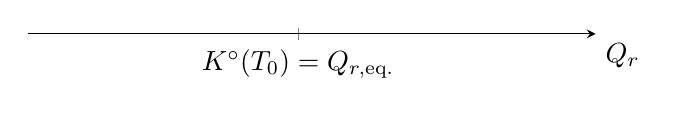
\begin{tikzpicture}
                \begin{axis}[clip = false, axis lines = left, axis line style={shorten >=-10pt}, axis y line=none, xmax=5, ymax=3, xmin=0, ymin=0, xtick={2.5},xticklabels={$K^\circ(T_0)=Q_{r,\equi}$}, ytick=\empty,  >=latex, xlabel=$Q_r$,every axis x label/.style={anchor=north east,at={(1.1,0)},xshift=10pt}]
                \end{axis}
            \end{tikzpicture}
            \end{figure}
            Après perturbation~:
            \begin{figure}[H]
            \centering
            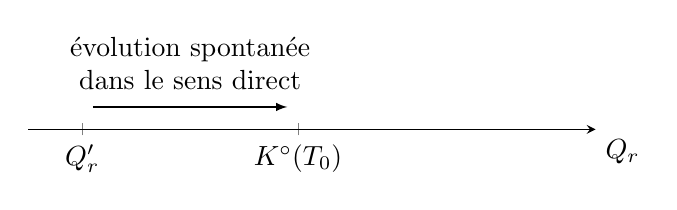
\begin{tikzpicture}
                \begin{axis}[clip = false, axis lines = left, axis line style={shorten >=-10pt}, axis y line=none, xmax=5, ymax=3, xmin=0, ymin=0, xtick={0.5,2.5},xticklabels={$Q_r'$,$K^\circ(T_0)$}, ytick=\empty,  >=latex, xlabel=$Q_r$,every axis x label/.style={anchor=north east,at={(1.1,0)},xshift=10pt}]
                    \draw [->] (0.6,0.15) --node [above, align=center,yshift=1mm]{évolution spontanée\\dans le sens direct} (2.4,0.15);
                \end{axis}
            \end{tikzpicture}
        \end{figure}
        En vertu du critère de l'évolution spontanée, le système évolue spontanément dans le sens direct, i.e. dans le sens d'une augmentation d'un nombre de moles gazeuses.\\
        \underline{Exemple~:} $\ce{2C_{(gr)} + O2_{(g)} = 2 CO_{(g)}}$. On a $\Dr \nu_{\gaz}=-1+2=+1>0$.
        \item \textbf{Second cas~: $\Dr \nu_{\gaz} <0$}\\
        On a donc $\frac{\dd{Q_r}}{Q_r}>0$ et donc $\dd{Q_r}>0$ d'où $Q_r \nearrow$.\\
        Initialement~:
        \begin{figure}[H]
            \centering
            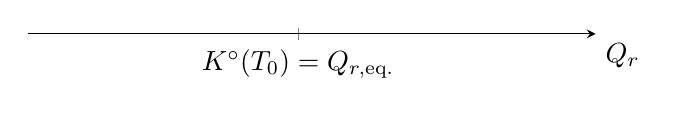
\begin{tikzpicture}
                \begin{axis}[clip = false, axis lines = left, axis line style={shorten >=-10pt}, axis y line=none, xmax=5, ymax=3, xmin=0, ymin=0, xtick={2.5},xticklabels={$K^\circ(T_0)=Q_{r,\equi}$}, ytick=\empty,  >=latex, xlabel=$Q_r$,every axis x label/.style={anchor=north east,at={(1.1,0)},xshift=10pt}]
                \end{axis}
            \end{tikzpicture}
            \end{figure}
            Après perturbation~:
            \begin{figure}[H]
            \centering
            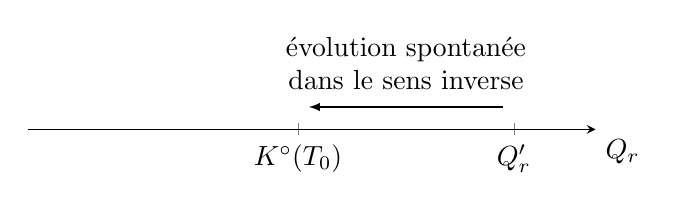
\begin{tikzpicture}
                \begin{axis}[clip = false, axis lines = left, axis line style={shorten >=-10pt}, axis y line=none, xmax=5, ymax=3, xmin=0, ymin=0, xtick={4.5,2.5},xticklabels={$Q_r'$,$K^\circ(T_0)$}, ytick=\empty,  >=latex, xlabel=$Q_r$,every axis x label/.style={anchor=north east,at={(1.1,0)},xshift=10pt}]
                    \draw [<-] (2.6,0.15) --node [above, align=center,yshift=1mm]{évolution spontanée\\dans le sens inverse} (4.4,0.15);
                \end{axis}
            \end{tikzpicture}
        \end{figure}
        En vertu du critère de l'évolution spontanée, le système évolue spontanément dans le sens inverse, i.e. dans le sens d'une augmentation d'un nombre de moles gazeuses.\\
        \underline{Exemple~:} $\ce{2 CO_{(g)}=2C_{(gr)} + O2_{(g)} }$. On a $\Dr \nu_{\gaz}=-2+1=-1<0$.
        \item \textbf{Troisième cas~: $\Dr \nu_{\gaz}=0$}\\
        On a $Q\neq 0$ donc $\dd{Q_r} = 0$.\\
        Donc l'ajout d'un constituant est sans effet sur le système qui demeure à l'équilibre.\\
        \underline{Exemple~:} $\ce{C_{(gr)} + O2_{(g)} = CO2_{(g)}}$. On a $\Dr \nu_{\gaz}=-1+1=0$.
    \end{itemize}
    CQDF.
\end{tableau}
\subsection{Ajout d’un constituant gazeux actif}
\subsubsection{Ajout isotherme et isochore}
\begin{enonce}
    L’introduction isotherme et isochore d’un constituant actif dans un système siège d’un équilibre chimique tend à déplacer cet équilibre dans le sens de la consommation de ce constituant.
\end{enonce}
\begin{tableau}
    \textbf{Démonstration avec tous les constituants gazeux}\\
    Initialement, d'après la Loi d'Action des Masses (LAM)~:
    $$Q_r = \prod_{i=1}^N a_i^{\nu_i} = \prod_{i=1}^N \left(\frac{x_iP}{P^\circ}\right)^{\nu_i}=\prod_{i=1}^N \left(\frac{n_iP}{nP^\circ}\right)^{\nu_i}=\prod_{i=1}^N \left(\frac{n_iRT}{P^\circ V}\right)^{\nu_i}$$
    On ajoute un constituant actif noté $B_j$ (de quantité de matière $n_j$) à $T,V$ fixés. Ainsi,
    \begin{align*}
        Q_r&=\left[\prod_{i=1}^N \left(\frac{n_iRT}{P^\circ V}\right)^{\nu_i}\right]\left(\frac{n_jRT}{P^\circ V}\right)^{\nu_j}\\
        &=\underbrace{\widetilde{\cste} \times \left(\frac{RT}{P^\circ V}\right)^{\nu_j}}_{\cste}\times n_j^{\nu_j}\\
        \implies \ln(Q_r) &= \ln(\cste) + \nu_j \ln(n_j)\\
        \implies \frac{\dd{Q_r}}{Q_r} = \nu_j\frac{\dd{n_j}}{n_j}
    \end{align*}
    Puisqu'on ajoute $B_j$, on a donc $\dd{n_j} >0$. De plus $Q_r >0$ donc on discerne ainsi deux cas~:
    \begin{itemize}
        \item \textbf{Premier cas~: $B_j$ est produit ($\nu_j>0$)}\\
        On a $\dd{Q_r}>0$ donc $Q_r \nearrow$.\\
        Initialement~:
        \begin{figure}[H]
            \centering
            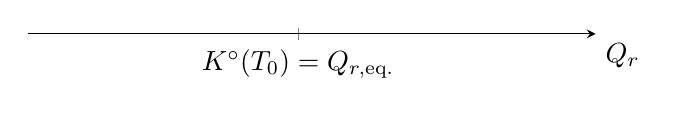
\begin{tikzpicture}
                \begin{axis}[clip = false, axis lines = left, axis line style={shorten >=-10pt}, axis y line=none, xmax=5, ymax=3, xmin=0, ymin=0, xtick={2.5},xticklabels={$K^\circ(T_0)=Q_{r,\equi}$}, ytick=\empty,  >=latex, xlabel=$Q_r$,every axis x label/.style={anchor=north east,at={(1.1,0)},xshift=10pt}]
                \end{axis}
            \end{tikzpicture}
            \end{figure}
            Après perturbation~:
            \begin{figure}[H]
            \centering
            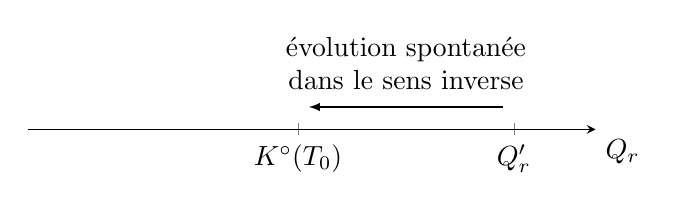
\begin{tikzpicture}
                \begin{axis}[clip = false, axis lines = left, axis line style={shorten >=-10pt}, axis y line=none, xmax=5, ymax=3, xmin=0, ymin=0, xtick={4.5,2.5},xticklabels={$Q_r'$,$K^\circ(T_0)$}, ytick=\empty,  >=latex, xlabel=$Q_r$,every axis x label/.style={anchor=north east,at={(1.1,0)},xshift=10pt}]
                    \draw [<-] (2.6,0.15) --node [above, align=center,yshift=1mm]{évolution spontanée\\dans le sens inverse} (4.4,0.15);
                \end{axis}
            \end{tikzpicture}
        \end{figure}
        En vertu du critère de l'évolution spontanée, le système évolue spontanément dans le sens inverse, i.e. dans le sens où $B_j$ est consommé.
        \item \textbf{Second cas~: $B_j$ est réactif ($\nu_j<0$)}\\
        On a $\dd{Q_r}<0$ donc $Q_r \searrow$.\\
        Initialement~:
        \begin{figure}[H]
            \centering
            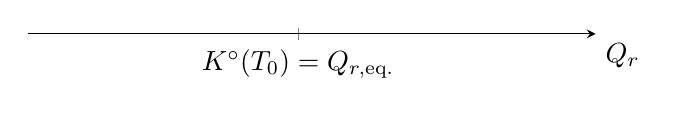
\begin{tikzpicture}
                \begin{axis}[clip = false, axis lines = left, axis line style={shorten >=-10pt}, axis y line=none, xmax=5, ymax=3, xmin=0, ymin=0, xtick={2.5},xticklabels={$K^\circ(T_0)=Q_{r,\equi}$}, ytick=\empty,  >=latex, xlabel=$Q_r$,every axis x label/.style={anchor=north east,at={(1.1,0)},xshift=10pt}]
                \end{axis}
            \end{tikzpicture}
            \end{figure}
            Après perturbation~:
            \begin{figure}[H]
            \centering
            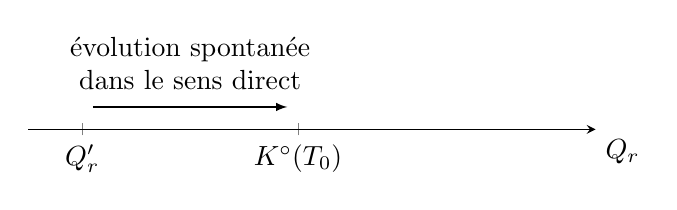
\begin{tikzpicture}
                \begin{axis}[clip = false, axis lines = left, axis line style={shorten >=-10pt}, axis y line=none, xmax=5, ymax=3, xmin=0, ymin=0, xtick={0.5,2.5},xticklabels={$Q_r'$,$K^\circ(T_0)$}, ytick=\empty,  >=latex, xlabel=$Q_r$,every axis x label/.style={anchor=north east,at={(1.1,0)},xshift=10pt}]
                    \draw [->] (0.6,0.15) --node [above, align=center,yshift=1mm]{évolution spontanée\\dans le sens direct} (2.4,0.15);
                \end{axis}
            \end{tikzpicture}
        \end{figure}
        En vertu du critère de l'évolution spontanée, le système évolue spontanément dans le sens direct, i.e. dans le sens où $B_j$ est consommé.
    \end{itemize}
    CQFD.
\end{tableau}

\subsubsection{Ajout isotherme et isobare}
L’introduction isotherme et isobare d’un constituant actif dans un système siège d’un équilibre chimique provoque une évolution du système qui dépend de la stoechiométrie de la réaction et de la nature (réactif ou produit) du constituant ajouté, et de l’état du système avant la perturbation.\\
Il est nécessaire à chaque fois d’étudier le signe de $\dd{\mathscr{A}}$ (variation élémentaire de l’affinité chimique) ou de $\dd{Q_r}$.
\end{document}
